\documentclass[a4paper,11pt]{article}
\usepackage[utf8]{inputenc}
\usepackage{graphicx}
\usepackage{float}

\graphicspath{ {./images/} }

\title{M2P4: Commitment Schemes}
\author{Joel Engström}

\begin{document}

\maketitle

\section{What is a Commitment Scheme?}
A commitment scheme allows an individual to \textit{commit} to a value before revealing it. They can then later share a secret which proves what the original message was, without also allowing them to change the message.

This serves an important purpose in multiple different areas of cryptography, not least zero-knowledge proofs.

\subsection{Our Commitment Scheme}

The commitment scheme considered here consists of a hash function where the input consists of a one bit long commit message concatenated with a 16 bit long random value \textit{k}. The output from the hash is then truncated to length \textit{X}.

\section{The Binding Property}
This property of a commitment scheme refers to the fact that once an original value has been chosen, it should not be possible to change that value. Thus, the sender has \textit{commited} to the original value chosen, and finding another value which gives the same output is generally thought of as being computationally unlikely.

\subsection{The Birthday Paradox}
The birthday paradox, in its most classical form, refers to the likelyhood that any two people in a group share the same birthday. Althouth the odds of this happening may initially seem low, they are in reality significantly higher than one would perhaps expect. This is due to the nature of the question asked: it is not a matter of if Alice has the same birthday as any other person in her class, but rather if any two people in the class share birthday. In fact, given a group size of just 23, it is more likely that there exists two people who share a birthday than not.

\subsection{How to Break the Binding Property}
Breaking the binding property means that the sender allows themselves to pretend to have encoded two different messages. They can therefore refrain from commiting to any one message beforehand. Finding multiple messages which compute to the same hash then allows the sender to choose between these previously chosen messages after the fact.

Utilizing the birthday paradox makes it significantly easier to break the binding property than one would otherwise assume. Since our commitment scheme encodes a single bit, we simply need to find any encoding of a zero-bit which gives the same output as any one encoding of a one-bit. Thus, this is not entirely unlike the birthday paradox.

A sender aiming to perform this attack would do so by finding two random values that would give the same hash for different encoded messages. They can then freely choose which value they want to pretend to have chosen.

\subsection{Probability of Breaking the Binding Property}
Breaking the binding property means finding two inputs which give the same hashed output for the first X bits. We calculate the probability that there exist two such identical values.

We define $ K $ as the number of possible permutations of \textit{k}:

\[ K = 2^{16} = 65536 \]

The odds of any permutation of K resulting in a match can be expressed as:

\[ P_{match}(X) = \frac{1}{2^{X}} \]

Seeing as this has to \textit{not} happen for all of our \textit{K} permutations, the probability that \textit{at least one} permutation results in a match can be expressed as:

\[ P(X) = 1 - (1 - \frac{1}{2^{X}})^{K} \]

\begin{figure}
  \begin{center}[H]
    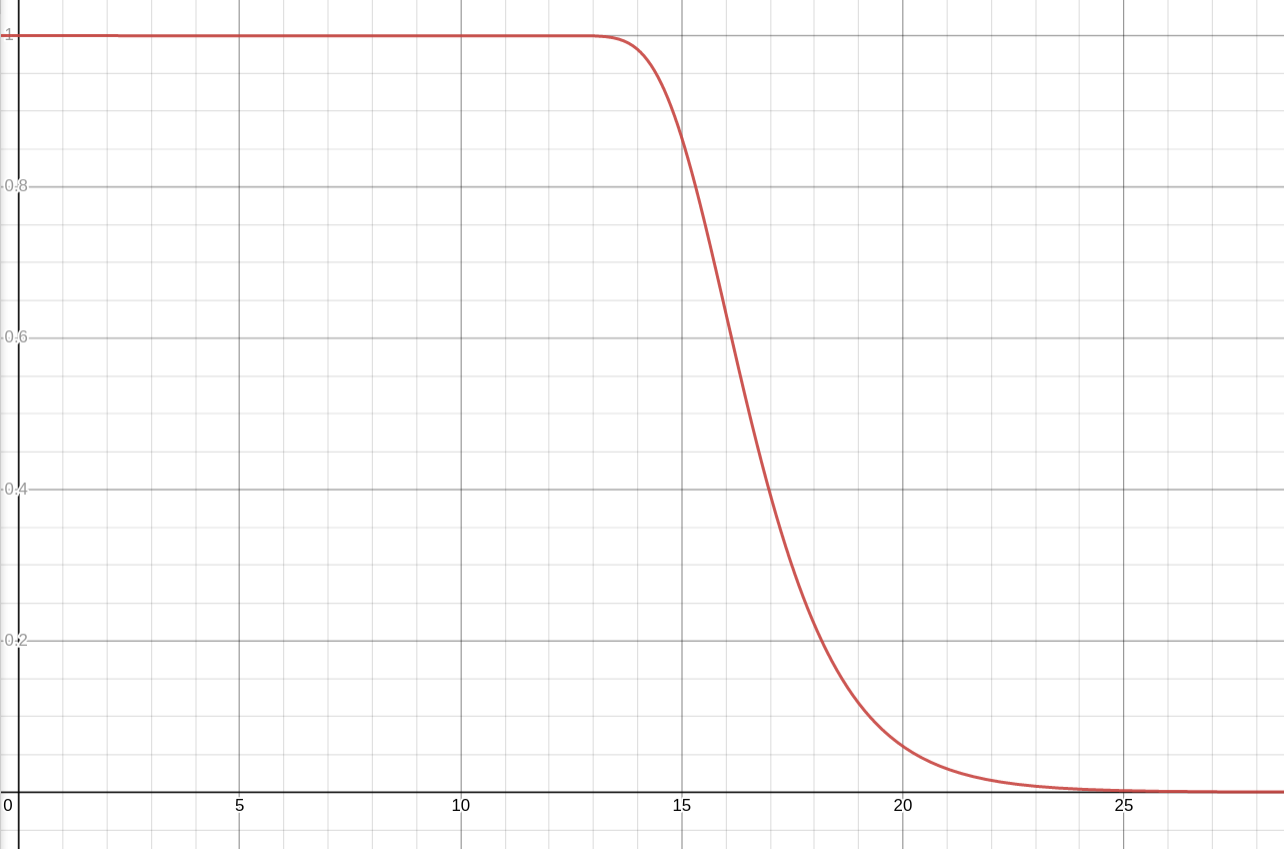
\includegraphics[width=0.7\linewidth]{binding.png}
    \caption{Probability of breaking the binding property as a function of the length of the truncated hash.}
    \label{fig:binding}
  \end{center}
\end{figure}

This figure shows a clear dropoff as the truncated hash length becomes longer.

\section{The Hiding Property}
Much like the binding property, the hiding property is a fundamental requirement for any commitment scheme to work. This means that one should not be able to calculate nor predict the input message through the output hash. The commitment scheme needs to utilize a one way hash function, meaning that a sufficient hash function should not be one that can be easily reversed. This is referred to as the \textit{preimage resistance} of a hash function.

\subsection{How to Break the Hiding Property}
Breaking the hiding property means, in this case, that the receiver is able to calculate or otherwise predict the input value bit, having access to only the output message. Since the hashing algorithm used can be assumed to have preimage resistance, the only way to break the hiding property would be to calculate hashes until you find a match.

\subsection{Probability of Breaking the Hiding Property}
Breaking the hiding property means calculating every single hash. $ 2^{16} $ possible random values, along with 2 possible message values (0 and 1) makes for a total of 
$ 2 * 2^{16} = 2^{17} $ values to hash.

The probability is, according to the assignment description, defined as:

\begin{quotation}
"For clarity, we define the probability of breaking the hiding property as the ratio between the number of possible x values for which the committed bit v can be uniquely determined and the total number of possible hash digests x output by the hash function."
\end{quotation}

We can determine the maximum number of uniquely determined values as $ 2^{X} $. Since we already know the total number possible hashes, we can express the complete probability as:

\[ P(X) = \frac{2^{X}}{2^{17}} \]

\begin{figure}
  \begin{center}[H]
    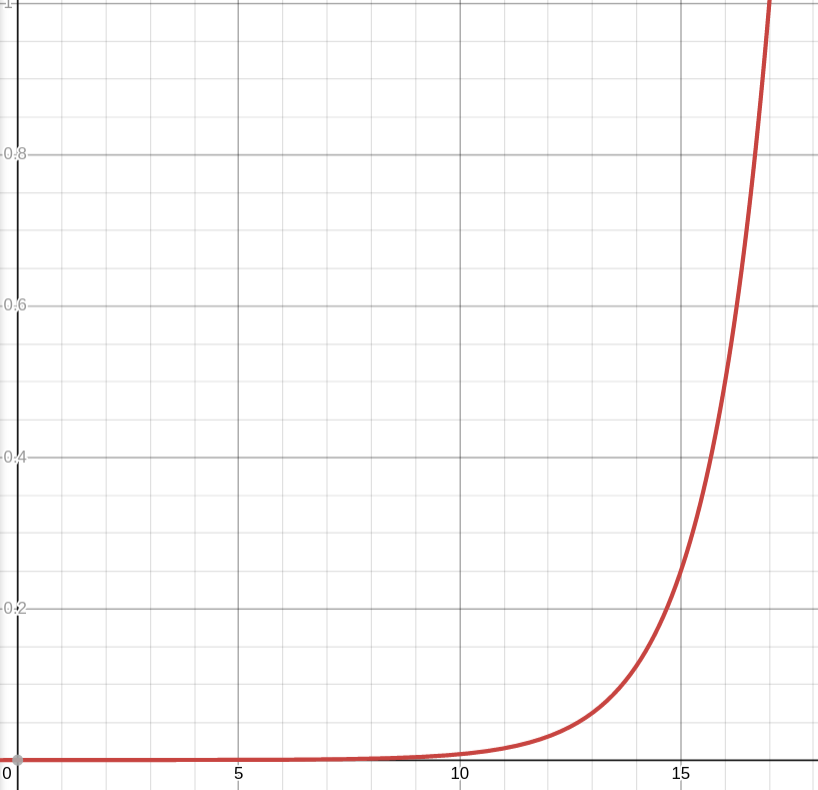
\includegraphics[width=0.7\linewidth]{hiding.png}
    \caption{Probability of breaking the hiding property as a function of the length of the truncated hash.}
    \label{fig:hiding}
  \end{center}
\end{figure}

The above figure clearly shows that as the truncation becomes longer, the attacker can be much more sure that the resulting input message they have is the correct one. Once the truncated length is equal to the original length of the total message to encode (16 random bits + 1 message bit), the attacker can be completely sure that their found message is correct.

\end{document}
